%----------------------------------------------------------------------------------------
%	Capítulo 5
%----------------------------------------------------------------------------------------

\pagestyle{myportland}
%\pagenumbering{arabic}
\doublespacing
\chapter[----- Diseño mecatrónico integral]{Diseño mecatrónico integral}
\thispagestyle{myportland}

%%%%%%%%%%%%%%%%%%%%%%%%%%%%%%%%%%%%%%%%%%%%%%%%%%%%%%%%%%%%%%
%%%%%                                                    %%%%%
%%%%%             DISEÑO MECATRÓNICO EN SÍ               %%%%%
%%%%%                                                    %%%%%
%%%%%%%%%%%%%%%%%%%%%%%%%%%%%%%%%%%%%%%%%%%%%%%%%%%%%%%%%%%%%%

%% NUEVA SECCIÓN X.X
\section{Desarrollo de diseño mecatrónico integral}

En la sección llamada \textit{"Desarrollo del diseño mecatrónico conceptual"} \cite{DiazVergara2020} se analizó el concepto de solución óptimo. En la Figura \ref{fig:estado diseno mecatronico etapa 3} se muestra la etapa final de unir las sub-soluciones para desarrollar una forma viable de implementarlos de una forma integral.

\begin{figure}[H]
	\centering
	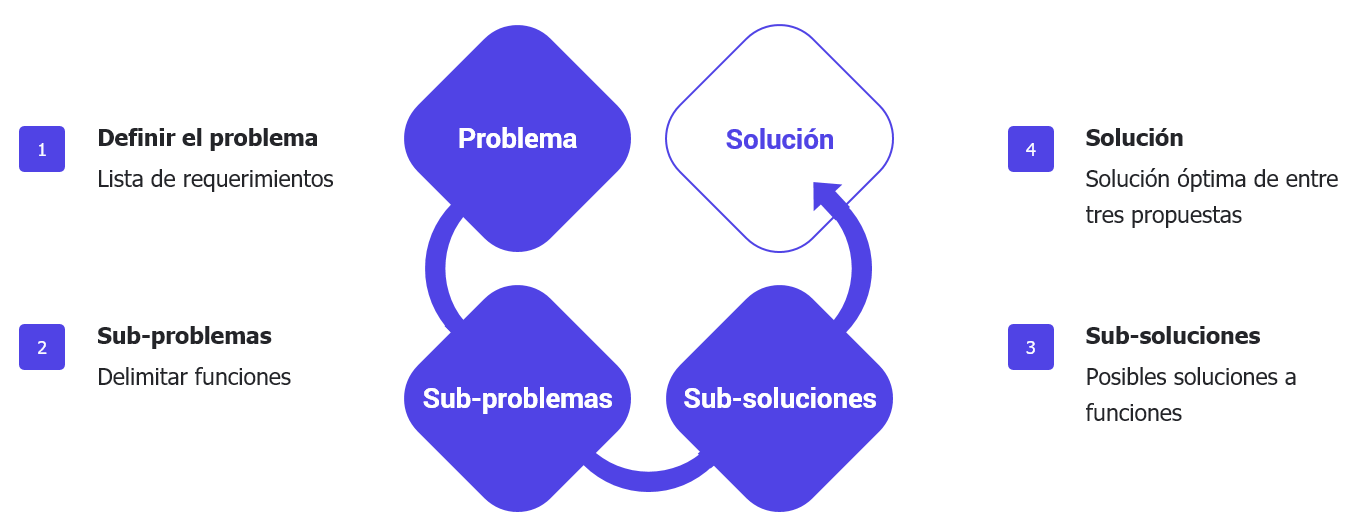
\includegraphics[width=1\textwidth]{chapter5/estado diseno subsoluciones.png}
	\caption{Estado de diseño mecatrónico: sub-soluciones}
	\begin{myflushleftportland}
		Fuente: Elaboración propia
	\end{myflushleftportland}
	\label{fig:estado diseno mecatronico etapa 3}
\end{figure}

\begin{figure}[H]
	\centering
	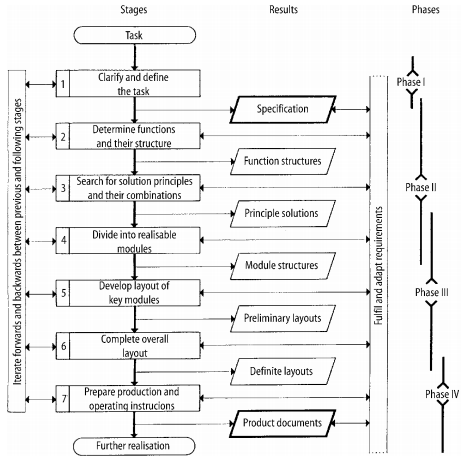
\includegraphics[width=0.75\textwidth]{chapter5/vdi2221.png}
	\caption{Fases de diseño según VDI 2221}
	\begin{myflushleftportland}
		Fuente: \cite{Pahl2007}
	\end{myflushleftportland}
	\label{fig:estado diseno mecatronico etapa 3}
\end{figure}

\begin{figure}[H]
	\centering
	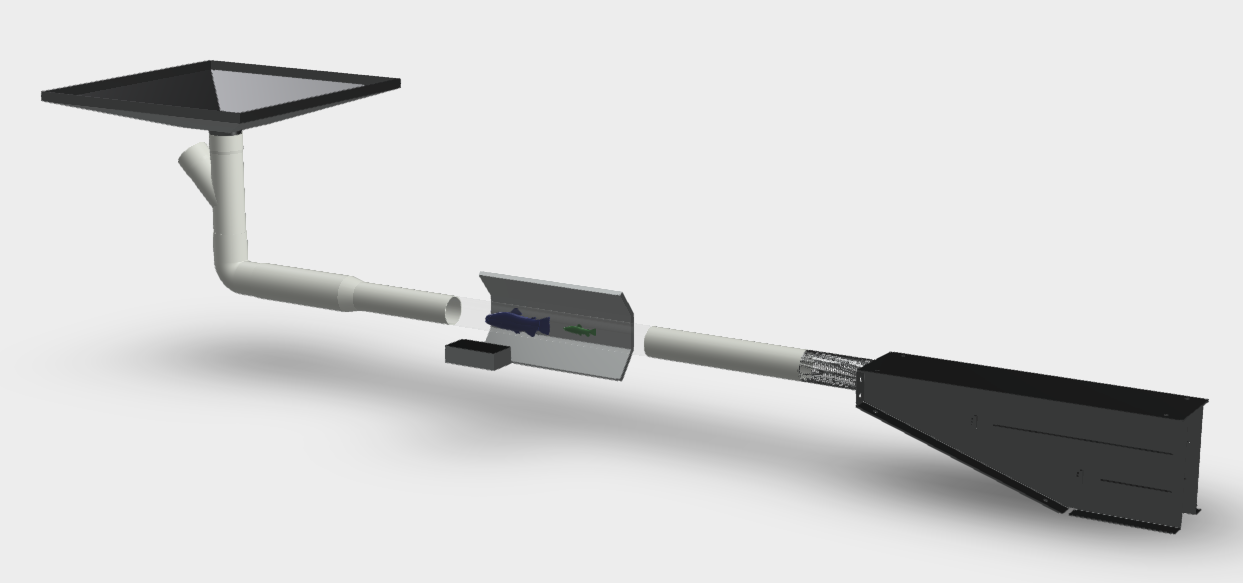
\includegraphics[width=1\textwidth]{chapter5/concepto optimo.png}
	\caption{Concepto óptimo}
	\begin{myflushleftportland}
		Fuente: Elaboración propia.
	\end{myflushleftportland}
	\label{fig:concepto optimo}
\end{figure}

%% NUEVA SECCIÓN X.X.X
\subsection{Descripción del sistema integral}

Dolor sit amet consectetur adipiscing elit ut aliquam purus sit. Dolor sed viverra ipsum nunc aliquet bibendum. Euismod in pellentesque massa placerat. Et malesuada fames ac turpis egestas sed tempus urna. Euismod elementum nisi quis eleifend quam adipiscing vitae proin. Ornare suspendisse sed nisi lacus sed. Mollis aliquam ut porttitor leo a diam.

%% NUEVO SUBSECCION X.X.X.X
\subsubsection{Arquitectura de hardware}

Dolor sit amet consectetur adipiscing elit ut aliquam purus sit. Dolor sed viverra ipsum nunc aliquet bibendum. Euismod in pellentesque massa placerat. Et malesuada fames ac turpis egestas sed tempus urna. Euismod elementum nisi quis eleifend quam adipiscing vitae proin. Ornare suspendisse sed nisi lacus sed. Mollis aliquam ut porttitor leo a diam.

%% NUEVO SUBSECCION X.X.X.X
\subsubsection{Selección de materiales de fabricación}

Dolor sit amet consectetur adipiscing elit ut aliquam purus sit. Dolor sed viverra ipsum nunc aliquet bibendum. Euismod in pellentesque massa placerat. Et malesuada fames ac turpis egestas sed tempus urna. Euismod elementum nisi quis eleifend quam adipiscing vitae proin. Ornare suspendisse sed nisi lacus sed. Mollis aliquam ut porttitor leo a diam.

%% NUEVA SECCIÓN X.X.X
\subsection{Subsistema de traslado de truchas}

Este subsistema consiste en encapsular los mecanismos físicos que están en el ciclo que sigue una trucha dentro de la máquina. 


%% NUEVO SUBSECCION X.X.X.X
\subsubsection{Diseño de tolvas}

\begin{itemize}
	
	\item \textbf{Diseño de tolva de recepción de truchas} 
	
	Lorem ipsum dolor sit amet, consectetur adipiscing elit, sed do eiusmod tempor incididunt ut labore et dolore magna aliqua. Lacus sed turpis tincidunt id aliquet. Nunc aliquet bibendum enim facilisis gravida neque convallis a. Ut tellus elementum sagittis vitae et leo duis ut diam. Dolor sit amet consectetur adipiscing elit ut aliquam purus sit. Dolor sed viverra ipsum nunc aliquet bibendum. Euismod in pellentesque massa placerat. Et malesuada fames ac turpis egestas sed tempus urna. Euismod elementum nisi quis eleifend quam adipiscing vitae proin. Ornare suspendisse sed nisi lacus sed. Mollis aliquam ut porttitor leo a diam. Varius morbi enim nunc faucibus. Sit amet purus gravida quis blandit turpis cursus in hac.
	
\end{itemize}



%% NUEVO SUBSECCION X.X.X.X
\subsubsection{Selección de reja accionada por motor}

Esta compuerta puede ser reemplazada por una tapa para la tolva de recepción de truchas. 

%% NUEVO SUBSECCION X.X.X.X
\subsubsection{Selección de bomba sumergible}

Lorem ipsum dolor sit amet, consectetur adipiscing elit, sed do eiusmod tempor incididunt ut labore et dolore magna aliqua. Lacus sed turpis tincidunt id aliquet. Nunc aliquet bibendum enim facilisis gravida neque convallis a. Ut tellus elementum sagittis vitae et leo duis ut diam. Dolor sit amet consectetur adipiscing elit ut aliquam purus sit. Dolor sed viverra ipsum nunc aliquet bibendum. Euismod in pellentesque massa placerat. Et malesuada fames ac turpis egestas sed tempus urna. Euismod elementum nisi quis eleifend quam adipiscing vitae proin. Ornare suspendisse sed nisi lacus sed. Mollis aliquam ut porttitor leo a diam. Varius morbi enim nunc faucibus. Sit amet purus gravida quis blandit turpis cursus in hac.

%% NUEVO SUBSECCION X.X.X.X


%% NUEVO SUBSECCION X.X.X.X




%% NUEVO SUBSECCION X.X.X.X
\subsubsection{Diseño de subsistema de distribución de truchas}

Luego del proceso de procesamiento de imágenes el sistema mediante el algoritmo de clasificación dirige a la trucha en tránsito a la salida correspondiente en el mecanismo de distribución de truchas. Dicho mecanismo recibe a la trucha y debe redirigir mediante un juego de compuertas a tres salidas que a su vez se impulsan mediante un caudal a sus respectivas jaulas flotantes.

\begin{itemize}
	
	\item \textbf{Cálculo de fuerza y velocidad de compuertas}
	La fuerza necesaria es simplemente el giro de la compuerta que está unida a un eje y a su vez al mecanismo de engranajes con el servomotor.
	
	\begin{figure}[H]
		\centering
		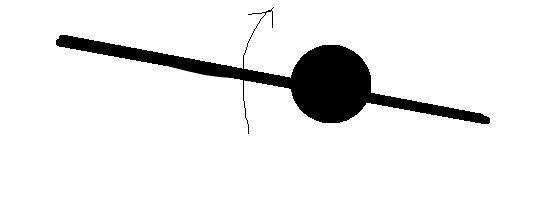
\includegraphics[width=1\textwidth]{chapter5/compuerta.png}
		\caption{Compuerta}
		\begin{myflushleftportland}
			Fuente: Elaboración propia.
		\end{myflushleftportland}
		\label{fig:compuerta}
	\end{figure}
	
	La velocidad de compuertas debe ir acorde a la distancia entre una trucha y la siguiente a esta. 
	
	\begin{figure}[H]
		\centering
		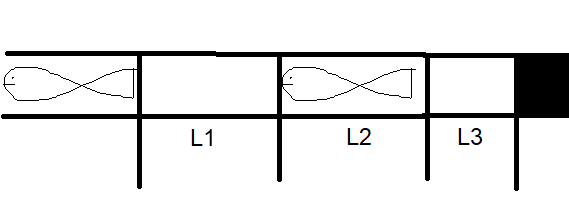
\includegraphics[width=1\textwidth]{chapter5/velocidad de compuerta.png}
		\caption{Velocidad de compuerta}
		\begin{myflushleftportland}
			Fuente: Elaboración propia.
		\end{myflushleftportland}
		\label{fig:velocidad de compuerta}
	\end{figure}

	Ut tellus elementum sagittis vitae et leo duis ut diam. Dolor sit amet consectetur adipiscing elit ut aliquam purus sit. 
	
	\begin{equation}\label{eq:calculo de tiempo necesario}
		\begin{split}
			L_1+L_2+L_3 &= t * v
		\end{split}		
	\end{equation}

	Ut tellus elementum sagittis vitae et leo duis ut diam. Dolor sit amet consectetur adipiscing elit ut aliquam purus sit. 

	
	\item \textbf{Selección de servomotores}
		
	Calcular: \\
	- Torque necesario \\
	- Condiciones de uso (estará en agua) \\
	- Tiempo de uso \\
	
	La selección de los servomotores depende del propósito en la función que se encuentre................
	
	\begin{itemize}
		
		%\item \textbf{Servomotor 1: } Este servomotor apoya en la función de \textit{accionar recepción de truchas}. 
		
		\item \textbf{Servomotor de compuerta}
		
		Este servomotor acciona la compuerta presentada en la Figura \ref{fig:compuerta}. El torque necesario del eje es $T_{max}=X (M*mm)$  y gracias al mecanismo de engranajes puede reducirse a $T_{max_2}=Y (M*mm)$ En la Tabla XXX se muestra una comparación técnica entre tres servomotores que cumplen los requerimientos técnicos y conceptuales.
		
	\end{itemize}


	\item \textbf{Diseño de mecanismo servomotor-compuerta} 
	
	Ut tellus elementum sagittis vitae et leo duis ut diam. Dolor sit amet consectetur adipiscing elit ut aliquam purus sit. 
	
	\begin{figure}[H]
		\centering
		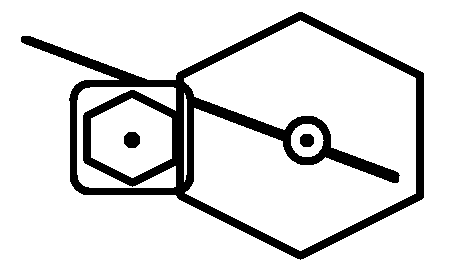
\includegraphics[width=1\textwidth]{chapter5/mecanismo servomotor-compuerta.png}
		\caption{Mecanismo servomotor-compuerta}
		\begin{myflushleftportland}
			Fuente: Elaboración propia.
		\end{myflushleftportland}
		\label{fig:mecanismo servomotor-compuerta}
	\end{figure}
	
	Ut tellus elementum sagittis vitae et leo duis ut diam. Dolor sit amet consectetur adipiscing elit ut aliquam purus sit. 
	
	\begin{figure}[H]
		\centering
		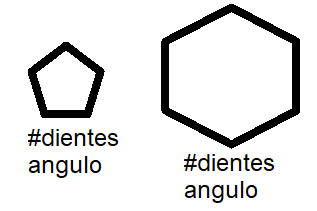
\includegraphics[width=1\textwidth]{chapter5/mecanismo de compuertas engranajes.png}
		\caption{Engranajes del mecanismo de compuertas}
		\begin{myflushleftportland}
			Fuente: Elaboración propia.
		\end{myflushleftportland}
		\label{fig:mecanismo de compuertas engranajes}
	\end{figure}
	
	Ut tellus elementum sagittis vitae et leo duis ut diam. Dolor sit amet consectetur adipiscing elit ut aliquam purus sit. 
	
	
	\item \textbf{Diseño de juego de compuertas programables}
	
	Descripción.

\end{itemize}



%% NUEVO SUBSECCION X.X.X.X
\subsubsection{Diseño de subsistema de tuberías}

Las tuberías del sistema tienen como propósito abastecer de un caudal a la máquina.

Lacus sed turpis tincidunt id aliquet. Nunc aliquet bibendum enim facilisis gravida neque convallis a. Ut tellus elementum sagittis vitae et leo duis ut diam. Dolor sit amet consectetur adipiscing elit ut aliquam purus sit. 

\begin{itemize}
	
	\item \textbf{Diseño de tuberías}
	
	Nunc aliquet bibendum enim facilisis gravida neque convallis a. Ut tellus elementum sagittis vitae et leo duis ut diam. Dolor sit amet consectetur adipiscing elit ut aliquam purus sit. Dolor sed viverra ipsum nunc aliquet bibendum. Euismod in pellentesque massa placerat. Et malesuada fames ac turpis egestas sed tempus urna. Euismod elementum nisi quis eleifend quam adipiscing vitae proin. Ornare suspendisse sed nisi lacus sed.
	
	\begin{figure}[H]
		\centering
		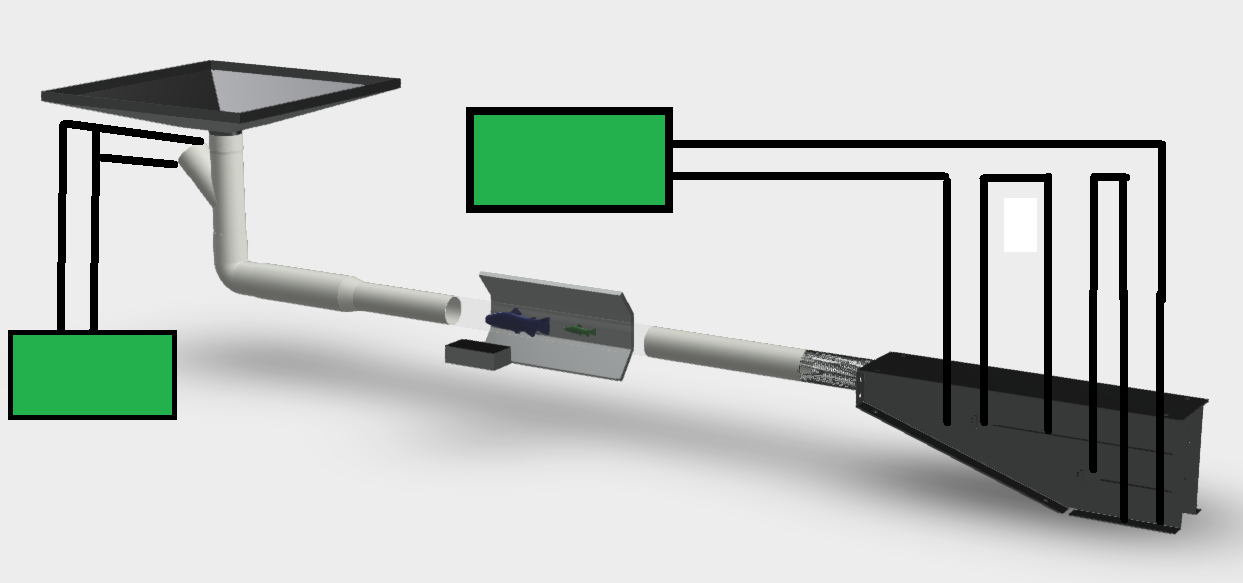
\includegraphics[width=1\textwidth]{chapter5/concepto optimo tuberias.png}
		\caption{Diseño de tuberías para el concepto óptimo}
		\begin{myflushleftportland}
			Fuente: Elaboración propia.
		\end{myflushleftportland}
		\label{fig:concepto optimo tuberias}
	\end{figure}

	Diseño de filtro único incluido
	
	Nunc aliquet bibendum enim facilisis gravida neque convallis a. Ut tellus elementum sagittis vitae et leo duis ut diam. Dolor sit amet consectetur adipiscing elit ut aliquam purus sit. Dolor sed viverra ipsum nunc aliquet bibendum. Euismod in pellentesque massa placerat. Et malesuada fames ac turpis egestas sed tempus urna. Euismod elementum nisi quis eleifend quam adipiscing vitae proin. Ornare suspendisse sed nisi lacus sed.	
	
	\begin{figure}[H]
		\centering
		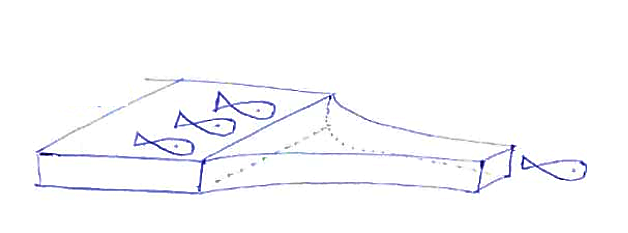
\includegraphics[width=0.25\textwidth]{chapter5/filtro unico.png}
		\caption{Filtro único}
		\begin{myflushleftportland}
			Fuente: Elaboración propia.
		\end{myflushleftportland}
		\label{fig:filtro unico}
	\end{figure}

	\item \textbf{Selección de caudales apropiados} 

	En la Sección \ref{sssec:seleccion de microcontrolador} se calculó la velocidad máxima, aproximada, de nado de las truchas arcoíris: $16 (cm/s)$. La Ecuación \ref{eq:calculo de caudal maximo} toma el valor de \textit{$v_{max}=16 (cm/s)$}  y el 
	
	\begin{equation}\label{eq:calculo de caudal maximo}
		\begin{split}
			Q_{max} & = v_{max}*A \\
			Q_{max} & = 16*\frac{\pi}{4}*(r_{int})^2 \\
			Q_{max} & = 16*\frac{\pi}{4}*(9.1)^2 \\
			Q_{max} & = 1040.62 \\
		\end{split}		
	\end{equation}
	Donde: $Q_{max} (cm^3/s)$ es el caudal máximo, $v_{max} (cm/s)$ es la velocidad máxima del agua, $r_{int} (cm)$
	
	Lorem ipsum dolor sit amet, consectetur adipiscing elit, sed do eiusmod tempor incididunt ut labore et dolore magna aliqua. Lacus sed turpis tincidunt id aliquet. Nunc aliquet bibendum enim facilisis gravida neque convallis a. Ut tellus elementum sagittis vitae et leo duis ut diam. Dolor sit amet consectetur adipiscing elit ut aliquam purus sit.	

	
	\item \textbf{Selección de las electroválvulas}
	
	Los valores límites que se tendrían que controlar mediante las electroválvulas pertenecen al rango $[0;12345] (m^3/s)$. En la Tabla XXX se muestran algunas marcas que cumplen con estos requerimientos.
	
	
	\begin{figure}[H]
		\centering
		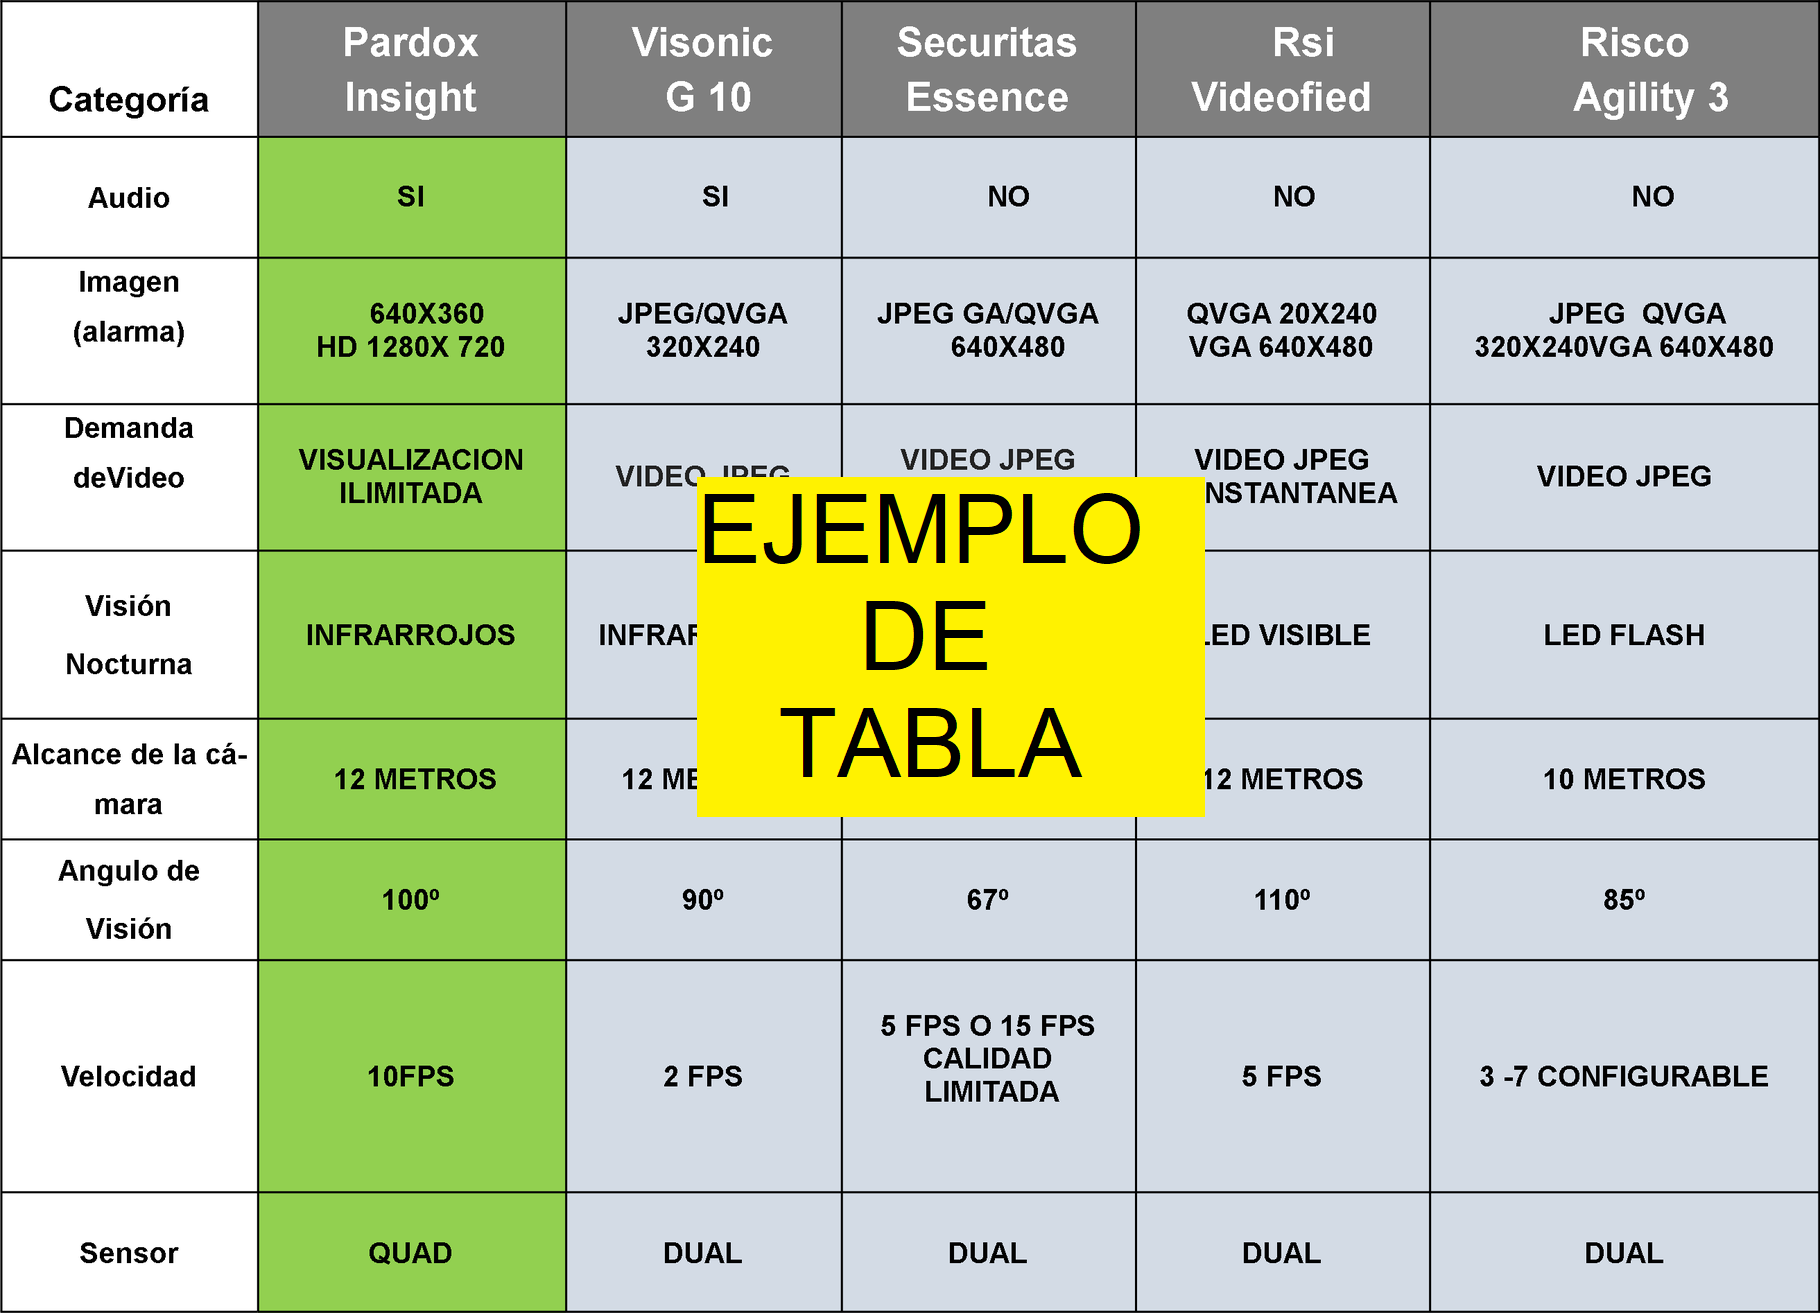
\includegraphics[width=0.85\textwidth]{chapter5/ejemplo de tabla.png}
		\caption{Ejemplo de tabla}
		\begin{myflushleftportland}
			Fuente: Elaboración propia.
		\end{myflushleftportland}
		\label{fig:ejemplo de tabla}
	\end{figure}
	
	Las características técnicas que se muestran en la Tabla XXX muestran que ................................
	
	Et malesuada fames ac turpis egestas sed tempus urna. Euismod elementum nisi quis eleifend quam adipiscing vitae proin. Ornare suspendisse sed nisi lacus sed. Mollis aliquam ut porttitor leo a diam. Varius morbi enim nunc faucibus. Sit amet purus gravida quis blandit turpis cursus in hac.
	
	\item \textbf{Control de los caudales de agua}
	
	Los caudales que generan las bombas de agua sirven para impulsar a las truchas por el interior de la máquina. 
	
	
	\begin{figure}[H]
		\centering
		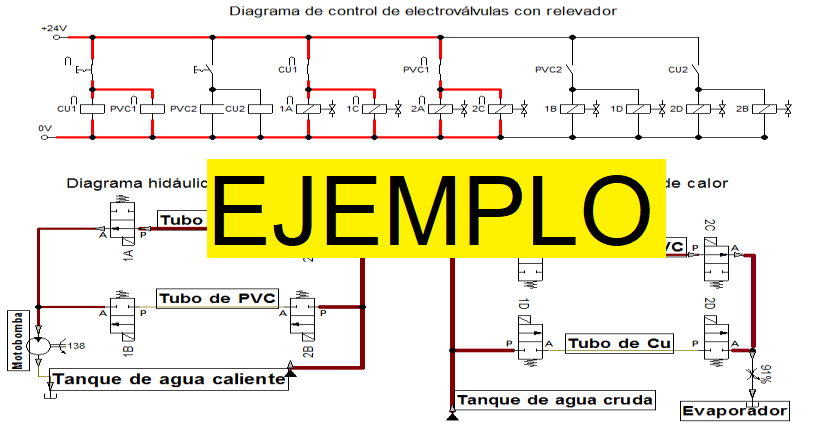
\includegraphics[width=1\textwidth]{chapter5/diagrama de control de electrovalvulas.png}
		\caption{Diagrama de control de electrovalvulas}
		\begin{myflushleftportland}
			Fuente: Elaboración propia.
		\end{myflushleftportland}
		\label{fig:diagrama de control de electrovalvulas}
	\end{figure}

	Lacus sed turpis tincidunt id aliquet. Nunc aliquet bibendum enim facilisis gravida neque convallis a. Ut tellus elementum sagittis vitae et leo duis ut diam. Dolor sit amet consectetur adipiscing elit ut aliquam purus sit. 
	
	\begin{figure}[H]
		\centering
		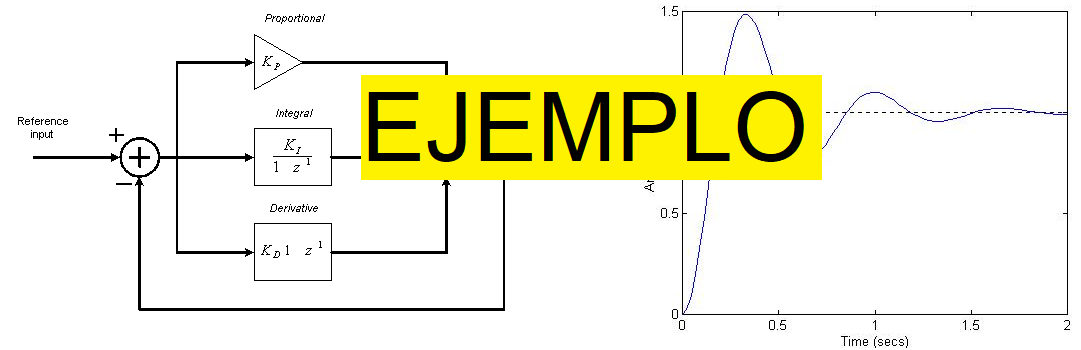
\includegraphics[width=1\textwidth]{chapter5/control electrovalvulas pid.png}
		\caption{Control PID de una electrovalvula}
		\begin{myflushleftportland}
			Fuente: Elaboración propia.
		\end{myflushleftportland}
		\label{fig:control electrovalvulas pid}
	\end{figure}
	
	Lacus sed turpis tincidunt id aliquet. Nunc aliquet bibendum enim facilisis gravida neque convallis a. Ut tellus elementum sagittis vitae et leo duis ut diam. Dolor sit amet consectetur adipiscing elit ut aliquam purus sit. 


\end{itemize}

%% NUEVA SECCIÓN X.X.X
\subsection{Subsistema de procesamiento de imágenes}

Este subsistema consiste obtener una serie de imágenes de una trucha en tránsito e indicar al sistema a dónde debería dirigirse una trucha determinada. El subsistema debe clasificar y contar truchas, con dicha finalidad necesita de la selección de una cámara y generar el ambiente adecuado para obtener las imágenes. Explicado los objetivos del subsistema, en las siguientes líneas se detalla: la selección del sensor infrarrojo, la selección de cámara estéreo, la selección de iluminación adecuada y la selección de algoritmos.

%% NUEVO SUBSECCION X.X.X.X
\subsubsection{Selección del sensor infrarrojo}
\label{sssec:seleccion del sensor infrarrojo}

El sensor infrarrojo tiene como objetivo activar el algoritmo de detección y conteo de truchas por un determinado periodo de tiempo con la finalidad de evitar un sobre uso de los recursos computacionales. El sensor infrarrojo está unos centímetros antes de la parte que la cámara captura y su posición es como se muestra en las Figura \ref{fig:posicion sensor infrarrojo}.

\begin{figure}[H]
	\centering
	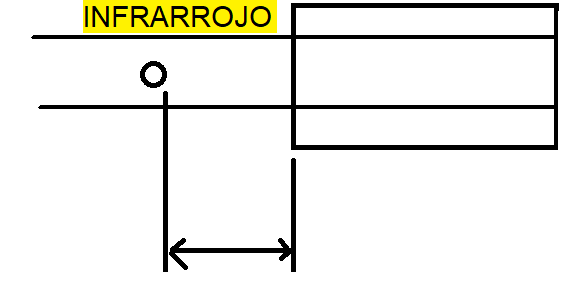
\includegraphics[width=1\textwidth]{chapter5/posicion sensor infrarrojo.png}
	\caption{Posicionamiento del sensor infrarrojo}
	\begin{myflushleftportland}
		Fuente: Elaboración propia.
	\end{myflushleftportland}
	\label{fig:posicion sensor infrarrojo}
\end{figure}

Entonces, el sensor infrarrojo debe tener un tiempo de respuesta ........ ........ Las comparaciones técnicas de los dispositivos comerciales que cumplen este requerimiento se muestran en la Tabla XXX.

\begin{figure}[H]
	\centering
	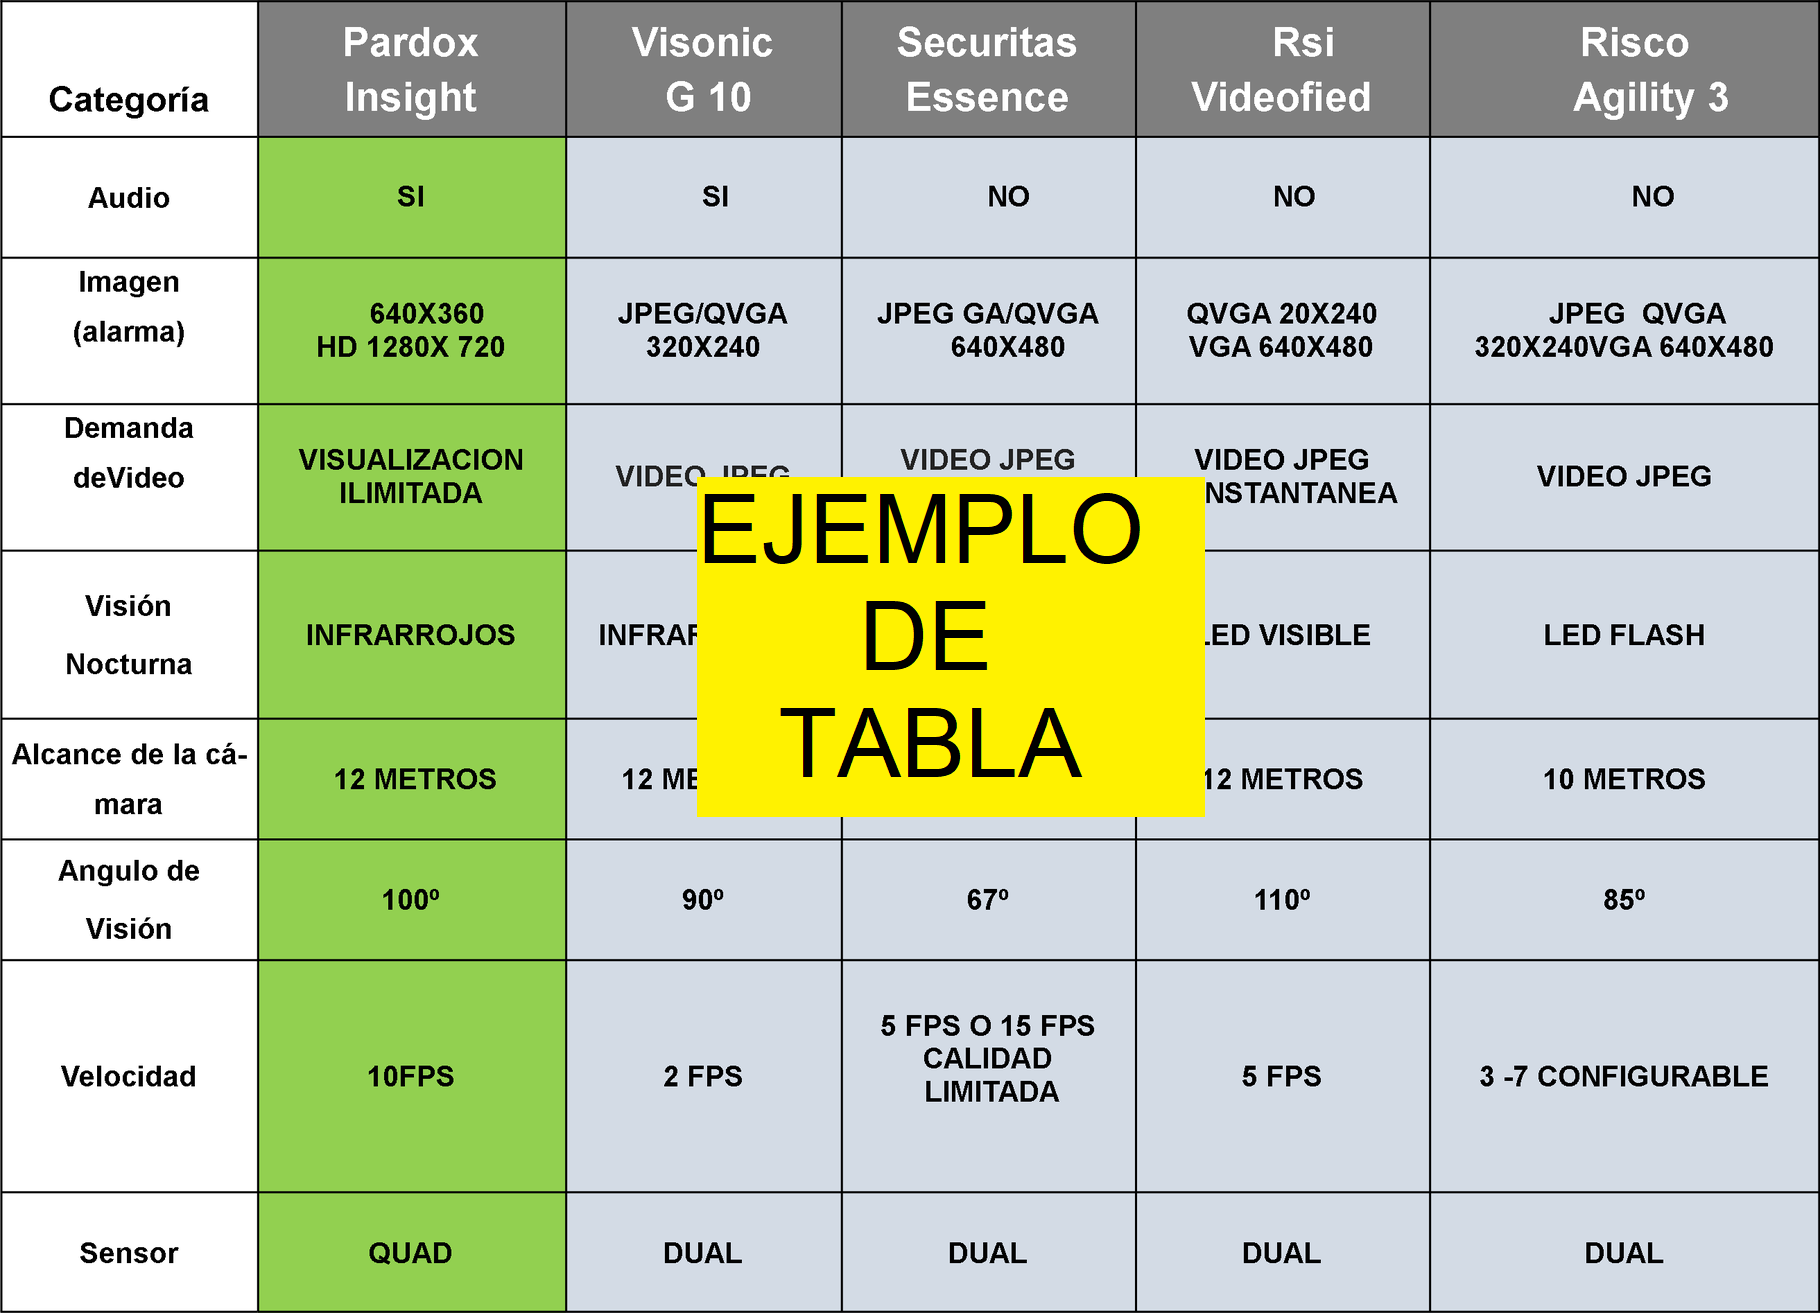
\includegraphics[width=0.85\textwidth]{chapter5/ejemplo de tabla.png}
	\caption{Ejemplo de tabla}
	\begin{myflushleftportland}
		Fuente: Elaboración propia.
	\end{myflushleftportland}
	\label{fig:ejemplo de tabla}
\end{figure}

%% NUEVO SUBSECCION X.X.X.X
\subsubsection{Selección de cámara estéreo} % de alta potencia
\label{sssec:seleccion de camara estereo}

Lorem ipsum dolor sit amet, consectetur adipiscing elit, sed do eiusmod tempor incididunt ut labore et dolore magna aliqua. Lacus sed turpis tincidunt id aliquet. Nunc aliquet bibendum enim facilisis gravida neque convallis a. Ut tellus elementum sagittis vitae et leo duis ut diam. Dolor sit amet consectetur adipiscing elit ut aliquam purus sit. Dolor sed viverra ipsum nunc aliquet bibendum. Euismod in pellentesque massa placerat. Et malesuada fames ac turpis egestas sed tempus urna. Euismod elementum nisi quis eleifend quam adipiscing vitae proin. Ornare suspendisse sed nisi lacus sed. Mollis aliquam ut porttitor leo a diam. Varius morbi enim nunc faucibus. Sit amet purus gravida quis blandit turpis cursus in hac.

Tener en cuenta: \\
- Tamaño de píxeles requerido \\
- Cantidad de frames (80 fps con 3-4L/s) (Falta calcular con lo que hemos calculado 16 cm/s) \\ 
- La inclinación hace que el pez no tenga velocidad hacia arriba \\
- Cámara estereo o simple?? \\
- Necesita GPU? \\

"TABLA X"

%% NUEVO SUBSECCION X.X.X.X
\subsubsection{Selección de iluminación adecuada} 
\label{sssec:seleccion de iluminacion adecuada}

Lorem ipsum dolor sit amet, consectetur adipiscing elit, sed do eiusmod tempor incididunt ut labore et dolore magna aliqua. Lacus sed turpis tincidunt id aliquet. Nunc aliquet bibendum enim facilisis gravida neque convallis a. Ut tellus elementum sagittis vitae et leo duis ut diam. Dolor sit amet consectetur adipiscing elit ut aliquam purus sit. Dolor sed viverra ipsum nunc aliquet bibendum. Euismod in pellentesque massa placerat. Et malesuada fames ac turpis egestas sed tempus urna. Euismod elementum nisi quis eleifend quam adipiscing vitae proin. Ornare suspendisse sed nisi lacus sed. Mollis aliquam ut porttitor leo a diam. Varius morbi enim nunc faucibus. Sit amet purus gravida quis blandit turpis cursus in hac.

%% NUEVO SUBSECCION X.X.X.X
\subsubsection{Selección de led de alta potencia} % de alta potencia
\label{sssec:seleccion de led de alta potencia}

El propósito de los leds de alta potencia es iluminar la zona en la que se realiza la captura de imágenes para detectar truchas y procesarlas. El uso de una led adecuado puede mejorar el rendimiento de la cámara.

Lorem ipsum dolor sit amet, consectetur adipiscing elit, sed do eiusmod tempor incididunt ut labore et dolore magna aliqua. Lacus sed turpis tincidunt id aliquet. Nunc aliquet bibendum enim facilisis gravida neque convallis a. Ut tellus elementum sagittis vitae et leo duis ut diam. Dolor sit amet consectetur adipiscing elit ut aliquam purus sit. Dolor sed viverra ipsum nunc aliquet bibendum. Euismod in pellentesque massa placerat. Et malesuada fames ac turpis egestas sed tempus urna. Euismod elementum nisi quis eleifend quam adipiscing vitae proin. Ornare suspendisse sed nisi lacus sed. Mollis aliquam ut porttitor leo a diam. Varius morbi enim nunc faucibus. Sit amet purus gravida quis blandit turpis cursus in hac.

%% NUEVO SUBSECCION X.X.X.X
\subsubsection{Selección de algoritmos}
\label{sssec:seleccion de algoritmos}

- NN: YOLO,YOLOv2,YOLOv3,YOLOv4,YOLOv5 \\
- NN: CNN - Fish segmentation \\
- Segmentación por características \\

Referencia a todas las versiones de YOLO. YOLO \cite{Redmon2016}, YOLO v2.0 \cite{Redmon2017}, YOLO v3.0 \cite{Redmon2018}, YOLO v4.0 \cite{Solawetz2020}, YOLO v5.0 \cite{bochkovskiy2020yolov4}.


\begin{itemize}
	
	\item \textbf{Selección de algoritmo contador de truchas:} Descripción.
	
	\item \textbf{Selección de algoritmo clasificador de truchas:} Descripción.
	
\end{itemize}

%% NUEVA SECCIÓN X.X.X
\subsection{Subsistema de suministro de energía}

 Dolor sit amet consectetur adipiscing elit ut aliquam purus sit. Dolor sit amet consectetur adipiscing elit ut aliquam purus sit. Dolor sit amet consectetur adipiscing elit ut aliquam purus sit.

%% NUEVO SUBSECCION X.X.X.X
\subsubsection{Selección de la batería} 

Ut tellus elementum sagittis vitae et leo duis ut diam. Dolor sit amet consectetur adipiscing elit ut aliquam purus sit.  Dolor sit amet consectetur adipiscing elit ut aliquam purus sit. las elementum sagittis vitae et.


%% NUEVO SUBSECCION X.X.X.X
\subsubsection{Selección de fuente de alimentación} 

Lorem ipsum dolor sit amet, consectetur adipiscing elit, sed do eiusmod tempor incididunt ut labore et dolore magna aliqua. Lacus sed turpis tincidunt id aliquet. Nunc aliquet bibendum enim facilisis gravida neque convallis a. Ut tellus elementum sagittis vitae et leo duis ut diam. Dolor sit amet consectetur adipiscing elit ut aliquam purus sit. Dolor sed viverra ipsum nunc aliquet bibendum. Euismod in pellentesque massa placerat. Et malesuada fames ac turpis egestas sed tempus urna. Euismod elementum nisi quis eleifend quam adipiscing vitae proin. Ornare suspendisse sed nisi lacus sed. Mollis aliquam ut porttitor leo a diam. Varius morbi enim nunc faucibus. Sit amet purus gravida quis blandit turpis cursus in hac.

%% NUEVO SUBSECCION X.X.X.X
\subsubsection{Selección de transformadores rectificadores}

Lorem ipsum dolor sit amet, consectetur adipiscing elit, sed do eiusmod tempor incididunt ut labore et dolore magna aliqua. Lacus sed turpis tincidunt id aliquet. Nunc aliquet bibendum enim facilisis gravida neque convallis a. Ut tellus elementum sagittis vitae et leo duis ut diam. Dolor sit amet consectetur adipiscing elit ut aliquam purus sit. Dolor sed viverra ipsum nunc aliquet bibendum. Euismod in pellentesque massa placerat. Et malesuada fames ac turpis egestas sed tempus urna. Euismod elementum nisi quis eleifend quam adipiscing vitae proin. Ornare suspendisse sed nisi lacus sed. Mollis aliquam ut porttitor leo a diam. Varius morbi enim nunc faucibus. Sit amet purus gravida quis blandit turpis cursus in hac.

%% NUEVO SUBSECCION X.X.X.X
\subsubsection{Selección de fuentes switching}

Lorem ipsum dolor sit amet, consectetur adipiscing elit, sed do eiusmod tempor incididunt ut labore et dolore magna aliqua. Lacus sed turpis tincidunt id aliquet. Nunc aliquet bibendum enim facilisis gravida neque convallis a. Ut tellus elementum sagittis vitae et leo duis ut diam. Dolor sit amet consectetur adipiscing elit ut aliquam purus sit. Dolor sed viverra ipsum nunc aliquet bibendum. Euismod in pellentesque massa placerat. Et malesuada fames ac turpis egestas sed tempus urna. Euismod elementum nisi quis eleifend quam adipiscing vitae proin. Ornare suspendisse sed nisi lacus sed. Mollis aliquam ut porttitor leo a diam. Varius morbi enim nunc faucibus. Sit amet purus gravida quis blandit turpis cursus in hac.


%% NUEVO SUBSECCION X.X.X.X
\subsubsection{Diagrama esquemático} 

Ut tellus elementum sagittis vitae et leo duis ut diam. Dolor sit amet consectetur adipiscing elit ut aliquam purus sit.


%% NUEVO SUBSECCION X.X.X.X
\subsubsection{Diagrama eléctrico} 

Ut tellus elementum sagittis vitae et leo duis ut diam. Dolor sit amet consectetur adipiscing elit ut aliquam purus sit.

%% NUEVA SECCIÓN X.X.X
\subsection{Subsistema de control e interacción con el usuario}

Nunc aliquet bibendum enim facilisis gravida neque convallis a. Ut tellus elementum sagittis vitae et leo duis ut diam. . Nunc aliquet bibendum enim facilisis gravida neque convallis a. Ut tellus elementum sagittis vitae et leo duis ut diam. 


%% NUEVO SUBSECCION X.X.X.X
\subsubsection{Selección de microcontrolador}
\label{sssec:seleccion de microcontrolador}

- Necesitamos: 80 fps \\
- Tamaño máximo: 15 cm \\
- Tamaño mínimo: 20 cm \\
- Velocidad estándar: 2 - 3 L/s (Longitud/segundos) \\
- Velocidad máxima: 3 - 4 L/s (Longitud/segundos) \\
- Debe poder: \\
---- procesar imágenes de forma rápida. \\
----  

En caso de usar NN \\
- 2 x Jetson Nano + Gumstix Jetson Nano Snapshot Board \\
- 1 x ESP32 \\

En caso de no usar NN \\
- ESP32 o Raspberry Pi 4B \\
- 1 x Jetson Nano \\

En la Sección \ref{sssec:algoritmos de deteccion de truchas}  se analiza los posibles algoritmos que pueden ser aplicados para la detección de truchas mediante visión por computadora.

Otros:\\
- Intel NSC2 \\

\begin{figure}[H]
	\centering
	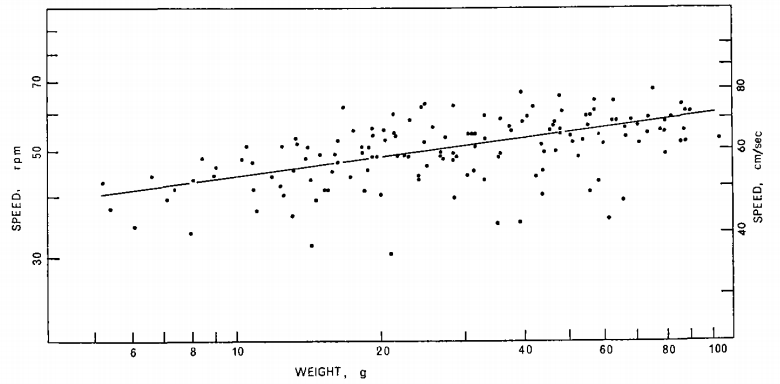
\includegraphics[width=1\textwidth]{chapter3/grafica tamano y velocidad de nado trucha arcoiris.png}
	\caption{Aproximación lineal de la relación entre peso y la velocidad de nado de truchas arcoíris}
	\begin{myflushleftportland}
		Fuente: \cite{Fry1970}
	\end{myflushleftportland}
	\label{fig:grafica tamano y velocidad de nado trucha arcoiris}
\end{figure}


En la Ecuación \ref{eq:ecuacion relacion tamano y velocidad de nado de trucha arcoiris} se muestra la relación entre \textit{X: peso de la trucha ($g$)} e \textit{Y: velocidad de nado ($cm/s$)} con un error \textit{Z= $\pm 0.033$}. 

\begin{equation} \label{eq:ecuacion relacion tamano y velocidad de nado de trucha arcoiris}
	Y=-3.965+2.908(Z)X
\end{equation}

En el caso de este trabajo, la dimensión máxima y mínima de las truchas arcoíris son de 20 cm y 15 cm, respectivamente. De la Tabla \ref{tbl:clasificacion de truchas por etapas de produccion} podemos obtener los gramos mediante interpolación lineal para cada límite: valores mínimo-máximo son 153 y 199 \textit{$g$}, respectivamente. Utilizando los valores antes indicados y empleando la Ecuación \ref{eq:ecuacion relacion tamano y velocidad de nado de trucha arcoiris} obtenemos los valores límites dentro del rango $[10.71; 15.13] (cm/s)$. Luego de escoger la máxima velocidad con redondeo hacia arriba (16 $cm/s$), ...


%% NUEVO SUBSECCION X.X.X.X
\subsubsection{Selección de indicadores visuales} % de alta potencia

Lorem ipsum dolor sit amet, consectetur adipiscing elit, sed do eiusmod tempor incididunt ut labore et dolore magna aliqua. Lacus sed turpis tincidunt id aliquet. Nunc aliquet bibendum enim facilisis gravida neque convallis a. Ut tellus elementum sagittis vitae et leo duis ut diam. Dolor sit amet consectetur adipiscing elit ut aliquam purus sit. Dolor sed viverra ipsum nunc aliquet bibendum. Euismod in pellentesque massa placerat. Et malesuada fames ac turpis egestas sed tempus urna. Euismod elementum nisi quis eleifend quam adipiscing vitae proin. Ornare suspendisse sed nisi lacus sed. Mollis aliquam ut porttitor leo a diam. Varius morbi enim nunc faucibus. Sit amet purus gravida quis blandit turpis cursus in hac.

%% NUEVO SUBSECCION X.X.X.X
\subsubsection{Selección de interruptor de seguridad de apagado de emergencia}

Lorem ipsum dolor sit amet, consectetur adipiscing elit, sed do eiusmod tempor incididunt ut labore et dolore magna aliqua. Lacus sed turpis tincidunt id aliquet. Nunc aliquet bibendum enim facilisis gravida neque convallis a. Ut tellus elementum sagittis vitae et leo duis ut diam. Dolor sit amet consectetur adipiscing elit ut aliquam purus sit. Dolor sed viverra ipsum nunc aliquet bibendum. Euismod in pellentesque massa placerat. Et malesuada fames ac turpis egestas sed tempus urna. Euismod elementum nisi quis eleifend quam adipiscing vitae proin. Ornare suspendisse sed nisi lacus sed. Mollis aliquam ut porttitor leo a diam. Varius morbi enim nunc faucibus. Sit amet purus gravida quis blandit turpis cursus in hac.

%% NUEVO SUBSECCION X.X.X.X
\subsubsection{Selección de interruptor de interruptor tipo hongo}

Lorem ipsum dolor sit amet, consectetur adipiscing elit, sed do eiusmod tempor incididunt ut labore et dolore magna aliqua. Lacus sed turpis tincidunt id aliquet. Nunc aliquet bibendum enim facilisis gravida neque convallis a. Ut tellus elementum sagittis vitae et leo duis ut diam. Dolor sit amet consectetur adipiscing elit ut aliquam purus sit. Dolor sed viverra ipsum nunc aliquet bibendum. Euismod in pellentesque massa placerat. Et malesuada fames ac turpis egestas sed tempus urna. Euismod elementum nisi quis eleifend quam adipiscing vitae proin. Ornare suspendisse sed nisi lacus sed. Mollis aliquam ut porttitor leo a diam. Varius morbi enim nunc faucibus. Sit amet purus gravida quis blandit turpis cursus in hac.

%% NUEVO SUBSECCION X.X.X.X
\subsubsection{Cálculo del consumo de energía del sistema} 

Ut tellus elementum sagittis vitae et leo duis ut diam. Dolor sit amet consectetur adipiscing elit ut aliquam purus sit.


%% NUEVO SUBSECCION X.X.X.X
\subsubsection{Diagrama de flujo}

Dolor sed viverra ipsum nunc aliquet bibendum. Euismod in pellentesque massa placerat. Et malesuada fames ac turpis egestas sed tempus urna. Euismod elementum nisi quis eleifend quam adipiscing vitae proin. Ornare suspendisse sed nisi lacus sed. Mollis aliquam ut porttitor leo a diam. Varius morbi enim nunc faucibus. Sit amet purus gravida quis blandit turpis cursus in hac.

%% NUEVO SUBSECCION X.X.X.X
\subsubsection{Diseño frontend de la aplicación móvil}

Lorem ipsum dolor sit amet, consectetur adipiscing elit, sed do eiusmod tempor incididunt ut labore et dolore magna aliqua. Lacus sed turpis tincidunt id aliquet. Nunc aliquet bibendum enim facilisis gravida neque convallis a. Ut tellus elementum sagittis vitae et leo duis ut diam. Dolor sit amet consectetur adipiscing elit ut aliquam purus sit. 


%% NUEVA SECCIÓN X.X.X
\subsection{Subsistema de flotadores}

%% NUEVO SUBSECCION X.X.X.X
\subsubsection{Cálculo de sistema flotador}

Lacus sed turpis tincidunt id aliquet. Nunc aliquet bibendum enim facilisis gravida neque convallis a. Ut tellus elementum sagittis vitae et leo duis ut diam. Dolor sit amet consectetur adipiscing elit ut aliquam purus sit. 

%% NUEVO SUBSECCION X.X.X.X
\subsubsection{Selección de flotadores}

Lacus sed turpis tincidunt id aliquet. Nunc aliquet bibendum enim facilisis gravida neque convallis a. Ut tellus elementum sagittis vitae et leo duis ut diam. Dolor sit amet consectetur adipiscing elit ut aliquam purus sit. 

%% NUEVO SUBSECCION X.X.X.X
\subsubsection{Diseño de sistema de flotadores}

Lacus sed turpis tincidunt id aliquet. Nunc aliquet bibendum enim facilisis gravida neque convallis a. Ut tellus elementum sagittis vitae et leo duis ut diam. Dolor sit amet consectetur adipiscing elit ut aliquam purus sit. 
